% #region PREAMBEL OG PAKKER
\documentclass[a4paper, 12pt]{article}  % DOKUMENTKLASSE
\title{Øving 9}                         % TITTEL
\author{Håvard Solberg Nybøe}           % FORFATTER
\date{MA0301}                           % DATO & FAG

\usepackage[english, norsk]{babel}      % NORSK SPRÅK
\usepackage[
    backend=biber,style=apa]{biblatex}  % BIBLIOGRAFI
\usepackage{csquotes}                   % PAKKE TIL BABEL
\addbibresource{bibliografi.bib}         % PATH TIL BIBLIOGRAFI
\usepackage[hidelinks]{hyperref}        % LENKER I TOC OG GENERELT
\usepackage[margin=1in]{geometry}       % VANLIG STØRRELSE MARGIN
\setlength{\parindent}{0em}             % SKILLER AVSNITT
\setlength{\parskip}{.8em}              % SKILLER AVSNITT
\usepackage{graphicx}                   % BILDER \includegraphics[OPTIONS]{PATH}
\usepackage{kantlipsum}                 % FYLLTEKST I KANT-STIL (kant[n-m])
\usepackage{amsfonts,                   % BLACKBOARD BOLD FONT (\mathbb{N})
amsmath,stmaryrd,amssymb}               % ANDRE MATTE PAKKER
\usepackage{circuitikz}                 % LOGISKE PORTER OG KRETSER & TikZ
\usepackage{import}                     % IMPORTER FILER (\import{PATH}{FILE})
\usepackage{caption}                    % PAKKE FOR BEDRE CAPTIONS I FIGURER
\usepackage{float}                       % FLYTT FIGURER 
% #endregion
\begin{document}

\maketitle
% \tableofcontents % INNHOLDSFORTEGNELSE

\begin{enumerate}
    \item [\boxed{1}]
    \begin{enumerate}
        \item 
        \begin{equation*}
            \left[
                \begin{array}{ccccc}
                    1 & 1 & 0 & 0 & 0 \\
                    0 & 1 & 1 & 0 & 1 \\
                    0 & 0 & 0 & 1 & 1 \\
                    1 & 0 & 1 & 1 & 0 \\
                    0 & 0 & 0 & 0 & 0
                \end{array}
            \right]
        \end{equation*}
        \begin{figure}[h!]
            \centering
            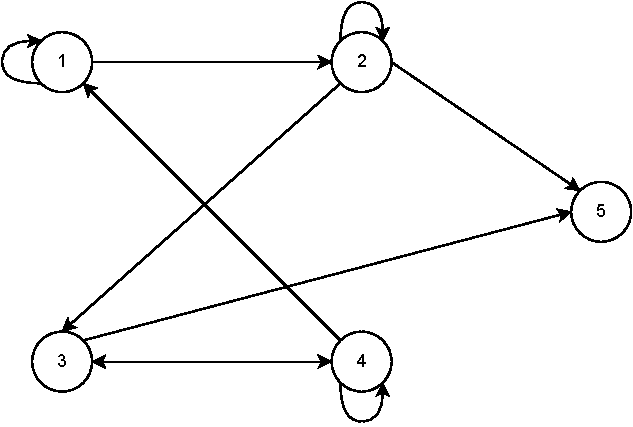
\includegraphics{graf1.pdf}
        \end{figure}
        \newpage
        \item 
        \begin{equation*}
            \left[
                \begin{array}{ccccc}
                    0 & 1 & 1 & 0 & 1 \\
                    1 & 0 & 0 & 1 & 1 \\
                    1 & 0 & 0 & 0 & 0 \\
                    0 & 1 & 0 & 0 & 1 \\
                    1 & 1 & 0 & 1 & 0
                \end{array}
            \right]
        \end{equation*}
        \begin{figure}[h!]
            \centering
            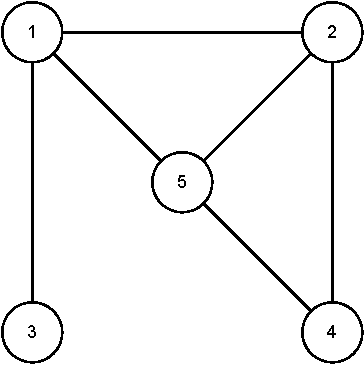
\includegraphics{graf2.pdf}
        \end{figure}
    \end{enumerate}
    \item [\boxed{2}]
    \begin{enumerate}
        \item 
    \end{enumerate}
\end{enumerate}

% \printbibliography[heading=bibintoc] % LAGER BIBLIOGRAFI
\end{document}
